\documentclass{beamer}
\usepackage{ulem}
\usepackage{tikz}
\usepackage{booktabs}
\usepackage{graphicx,threeparttable,caption}
\usetikzlibrary{shapes,snakes}
\usepackage[beamer,customcolors]{hf-tikz}
\usepackage{nicematrix}
\usepackage{xcolor}
\usepackage{makecell}
\usepackage{array}
\usepackage{csquotes}
\usepackage{csquotes}
\usepackage{minted}
\usepackage{animate}
\captionsetup{labelformat=empty,labelsep=none}

\graphicspath{ {./png/} }

\usetikzlibrary{
    arrows,
    arrows.meta,
    shapes,
    positioning,
    shadows,
    trees,
    calc
}

\tikzset{%
    >={Latex[width=2mm,length=2mm]},
    % Specifications for style of nodes:
    plain/.style = {},
    base/.style = {
        plain,
        rectangle, rounded corners, draw=black,
        minimum width=1cm, minimum height=1cm,
        text centered, font=\sffamily\tiny\bfseries,
        fill=white, align=center
    },
    app/.style = {base, ellipse},
    data/.style = {base, fill=gray!30},
    action/.style = {base, circle, fill=red!30},
    note/.style = {app, fill=yellow},
    hl/.style={
    set fill color=red!80!black!40,
    set border color=red!80!black
    }
}


\AtBeginSection[]{
  \begin{frame}
  \vfill
  \centering
  \begin{beamercolorbox}[sep=8pt,center,shadow=true,rounded=true]{title}
    \usebeamerfont{title}\insertsectionhead\par%
  \end{beamercolorbox}
  \vfill
  \end{frame}
}
\setbeamercolor{alerted text}{fg=red}
%\usecolortheme[orchid]{structure}
\usetheme[hideothersubsections]{PaloAlto}
\makeatletter
\patchcmd{\csq@bquote@i}{{#6}}{{\emph{#6}}}{}{}
\makeatother
%\usecolortheme{orchid}
%\usefonttheme{professionalfonts}
\newcommand{\soutthick}[1]{%
   \textcolor{red}{
   \renewcommand{\ULthickness}{1pt}%
      \sout{#1}%
   \renewcommand{\ULthickness}{.4pt}% Resetting to ulem default
   }
}
\newcommand{\centered}[1]{\begin{tabular}{l} #1 \end{tabular}}
\setbeamertemplate{section in toc}[square]
\setbeamertemplate{subsection in toc}[square]
\setbeamertemplate{section in sidebar}[shaded]
\setbeamertemplate{items}[square]
\setbeamercovered{transparent} 

\title[]{Introduction to Computational Social Science}
\subtitle{Computer simulation -- why simulate?}
\author[]{Mikołaj Biesaga\\ \small{\color{blue}{\href{mailto:m.biesaga@uw.edu.pl}{m.biesaga@uw.edu.pl}}}}
\institute{
\includegraphics[width = 4 cm]{uw.png}}
\date{April 15, 2025}
\begin{document}
\begin{frame}
   \titlepage
\end{frame}
\section[Models]{Models}
\begin{frame}
   \frametitle{What is a model?}
   \only<1>{
      \begin{figure}
         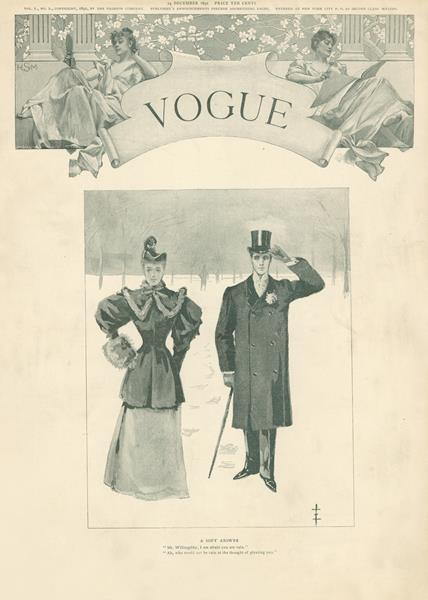
\includegraphics[width = .48\textwidth]{vogue.jpg}
         \caption{from \href{https://archive.vogue.com/issue/18921224}{\textcolor{blue}{Vogue}} (December 24, 1892)}

      \end{figure}
   }
   \only<2>{
      \begin{block}{Model}
         In simple terms a model is a \underline{simplified} representation of a system (reality) that helps to understand how the system works/worked in the past/will work in the future.
      \end{block}
   }
   \only<3,4>{
      \begin{itemize}
         \item What is a model? \href{https://youtu.be/RK9m4OmFAbY?feature=shared}{\textcolor{blue}{YouTube video}}
         \item<4> Formalizing a theory into a model allows the researcher to
         describe their ideas in a precise, unambiguous way (Goldstone \& Janssen 2005; Epstein 2008). 
         \item<4> Models are conceptually precise, their assumptions are clear;
         they allow formal deduction and an easy way to verify their internal
         validity (Timpone \& Taber 1996). 
         \item<4> Last but not least they provide an unambiguous way to
         communicate within the scientific community (Nowak, Rychwalska, \&
         Borkowski, 2015).
      \end{itemize}
      %% \begin{itemize}
      %%    \item What is a model? \href{https://www.youtube.com/watch?v=uWuNfhDvZz8}{\textcolor{blue}{YouTube video}}
      %% \end{itemize}
   }
   \only<5>{
      \framesubtitle{Simulating}
      \begin{tikzpicture}
         \node [text width = 1.5cm] at (0,0) {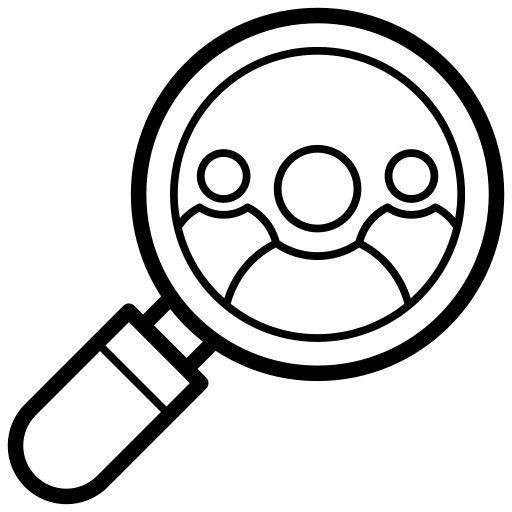
\includegraphics[width = \textwidth]{observation.png}};
         \node at (0,-2) {\footnotesize\textsc{Observation}};
         \node [text width = 1.5cm] at (2.5,0) {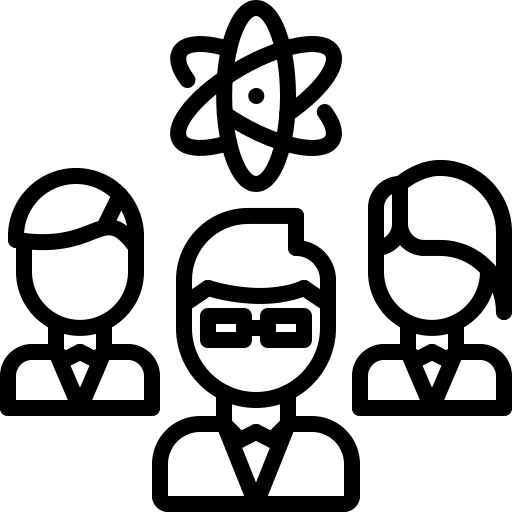
\includegraphics[width = \textwidth]{theory_formulation.png}};
         \node [text width = 2cm, align = center] at (2.5,-2) {\footnotesize\textsc{Theory \\Formulation}};
         \node [text width = 1.5cm] at (5,0) {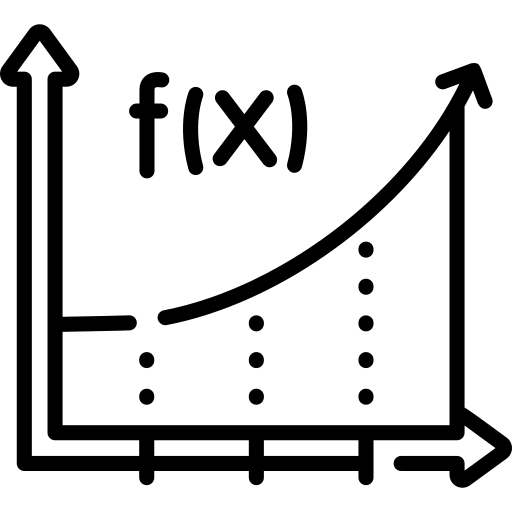
\includegraphics[width = \textwidth]{modeling.png}};
         \node [text width = 1.5cm, align = center] at (5,-2) {\footnotesize\textsc{Model \\Creation}};
         \node [text width = 1.5cm] at (7.5,0) {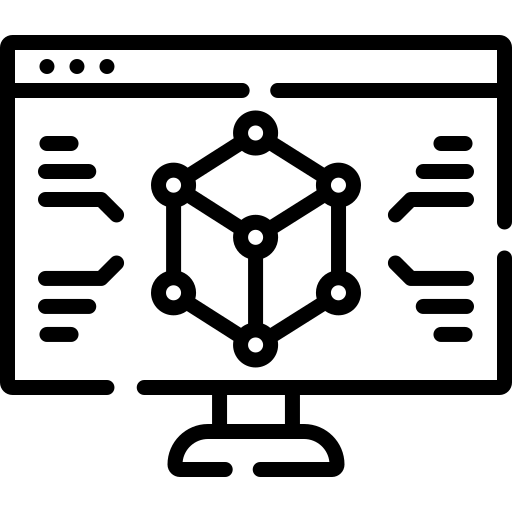
\includegraphics[width = \textwidth]{simulation.png}};
         \node at (7.5,-2) {\footnotesize\textsc{Simulating}};
         \draw [thick, ->] (.8,0) -- (1.7,0);
         \draw [thick, ->] (3.3,0) -- (4.2,0);
         \draw [thick, ->] (5.8,0) -- (6.7,0);
      \end{tikzpicture}
   }
   \only<6>{
      \framesubtitle{What are computer simulations?}
      \begin{block}{Computer Simulation}
         Computer simulation is the running of a model on a computer, the model
         being designed to represent the behaviour of, or the outcome of, a
         real-world or physical system. The reliability of some models
         can be determined by comparing their results to the real-world outcomes
         they aim to predict/explain.
      \end{block}
   }

\end{frame}
\section[Why simulate?]{Why simulate?}
\begin{frame}
   \frametitle{Why simulate?}
   \framesubtitle{Nowak, Rychwalska, \& Borkowski, 2015}
   \begin{enumerate}
      \item What is a mental model?
      \only<2>{
         \begin{itemize}
            \item "Mental models are the mind's replicas of phenomena, upon
            which humans manipulate to learn the mechanism and workings of the
            surrounding environment." (Ibidem, p.~2)
            \item Mental models develop most accurately through interaction with
            the target system (Norman, 1983).
         \end{itemize}
      }
      \item What are the benefits of simulating for scientists?
   \end{enumerate}
\end{frame}

\section[Agent-based models]{Agent-based models}
\begin{frame}
   \frametitle{Agent-based models}
   \only<1>{
      \begin{figure}
         \centering
         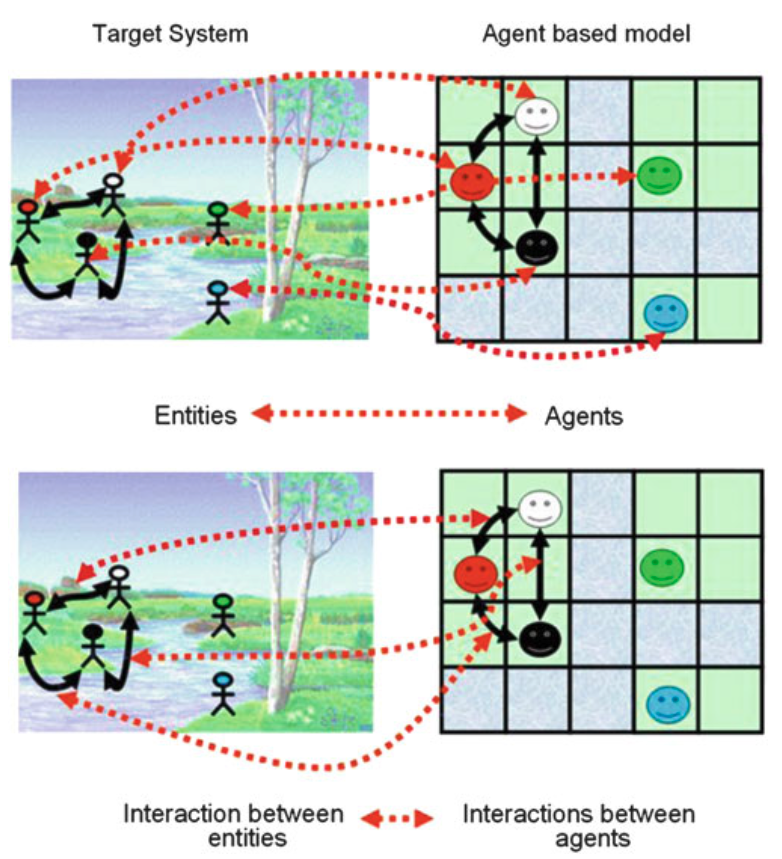
\includegraphics[width = .6\textwidth]{agent_based_models.png}
         \caption{Galan et al., 2013}
      \end{figure}
   }
   \only<2>{
      \begin{block}{Agent-based models}
         Agent-based models are discrete-time computer simulations used to study
         the interactions between people, things, places, and time. They are
         stochastic models built from the bottom up meaning individual agents
         (often people in epidemiology) are assigned certain attributes.
         \alert{The agents are programmed to behave and interact with other
         agents and the environment in certain ways.} These interactions produce
         emergent effects that may differ from effects of individual agents.
      \end{block}
   }
   \only<3>{
      \frametitle{Cellular automata}
      \begin{figure}
         \centering
         
\includegraphics[width = .9\textwidth]{grid.png}
      \end{figure}
   }
   \only<4>{
      \frametitle{Cellular automata}
      \framesubtitle{Game of life (Conway, 1970)}
      \begin{figure}
         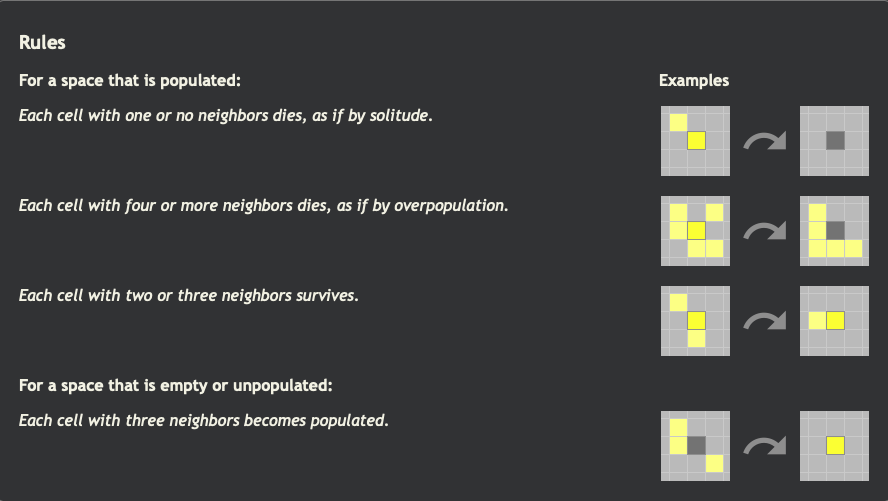
\includegraphics[width = .9\textwidth]{life.png}
      \end{figure}

   }
   \only<5>{
      \frametitle{Cellular automata}
      \framesubtitle{Game of life (Conway, 1970)}
      \begin{figure}
         \animategraphics[loop,controls, width = .9\textwidth]{10}{game_life-}{0}{148}
         \caption{from \href{https://playgameoflife.com}{\textcolor{blue}{https://playgameoflife.com}}}
      \end{figure}

   }
\end{frame}

\section[Models of segregation]{Models of segregation}
\begin{frame}
   \frametitle{Dynamic models of segregation}
   \framesubtitle{Schelling, 1971}
   \only<1>{
      \begin{itemize}
      \item In 1965, the last of \href{https://en.wikipedia.org/wiki/Jim_Crow_laws}{\textcolor{blue}{Jim Crow's}} racial segregation laws were overturned.
      \item Despite much effort and investment, segregation still remains a major issue in the U.S. and elsewhere to this date (Cassidy, 2016).
      \item "If an individual is surrounded by more individuals of different type than the number of individuals of own type, then the individual moves from the current location to a random empty location." (Schelling, 1971)
   \end{itemize}
   }
   \only<2,3>{
      \begin{figure}
      \centering
      \includegraphics<2,3>[width = \textwidth]{schelling1.png}
      \includegraphics<3>[width = \textwidth]{schelling2.png}
      \caption{Schelling, 1971}
      \end{figure}
   }

\end{frame}

\begin{frame}
   \frametitle{The world of polygons}
   \begin{figure}
      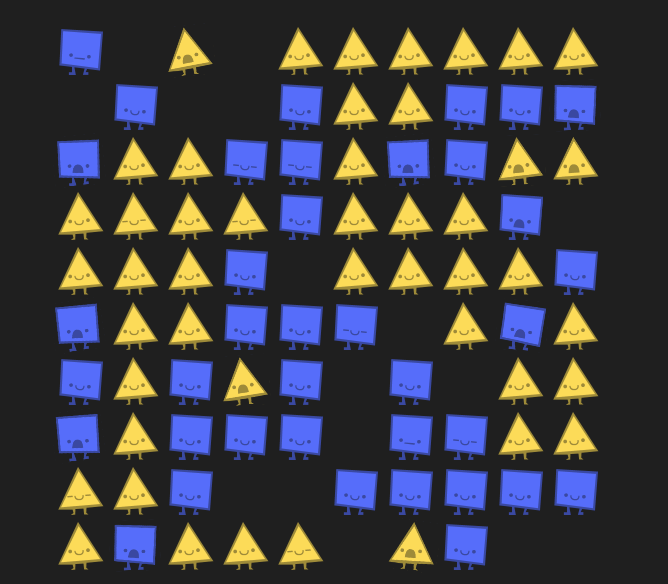
\includegraphics[width = .7\textwidth]{polygons.png}
      \caption{by Nicky Case from \href{https://ncase.me/polygons/}{\textcolor{blue}{https://ncase.me/polygons/}}}
   \end{figure}

\end{frame}

\begin{frame}
   \frametitle{\large Modeling Dynamics of Multicultural Integration and Conflict}
   \framesubtitle{de Raad, Nowak, \& Borkowski, 2013}
   \only<1,2>{
      \only<1>{
         \begin{itemize}
            \item Acculturation vs Segregation.
            \item A positive attitude means that contact with that person increases happiness, a negative attitude is related to a decrease.
            \item Although happiness increases with the number of positively valued contacts, this increase is not linear.
            \item Individuals, or agents, were assigned to a group, and given an attitude towards the own and other group ranging from $-1$ to $+1$.
            \item A decision to move would be made if a spot would provide a higher level of happiness than the current location.
         \end{itemize}
      }
      \only<2>{
         $$H = A_{own} \times \sqrt{N_{own}} + A_{other} \times \sqrt{N_{other}}$$
      }
   }
   \only<3>{
      \begin{figure}
         \begin{minipage}{.49\textwidth}
            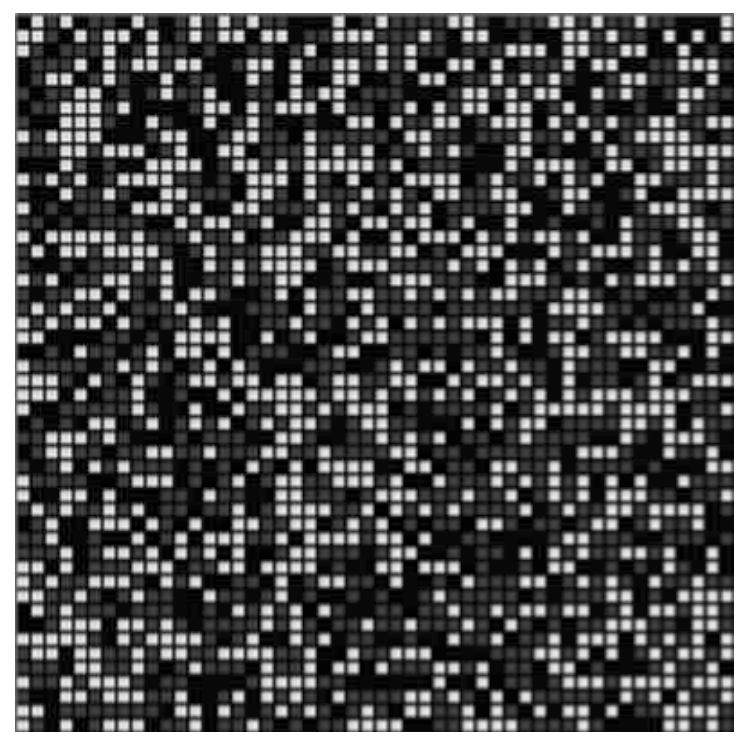
\includegraphics[width = \textwidth]{wouter1.png}
         \end{minipage}
         \begin{minipage}{.49\textwidth}
            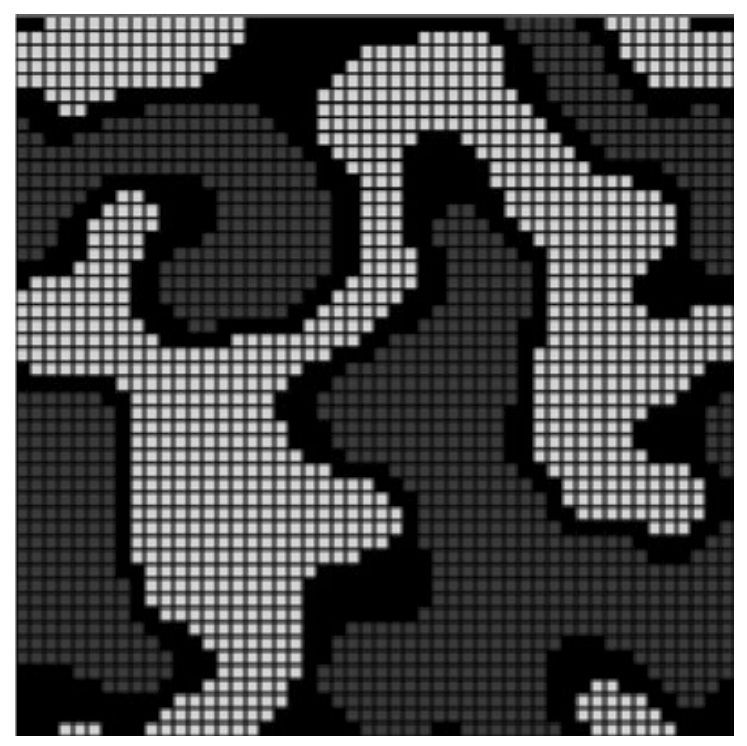
\includegraphics[width = \textwidth]{wouter2.png}
         \end{minipage}
         \caption{\footnotesize\textbf{Left panel:} Initial state of a
         simulation in which agents of two groups – depicted in two shades of
         gray are randomly distributed on a grid.  Black color indicates empty
         spaces to which agents can potentially move. \textbf{Right panel:}
         Pattern of intergroup contact between agents with mutual negative
         attitudes.}
      \end{figure}
   }
   \only<4>{
      \begin{figure}
         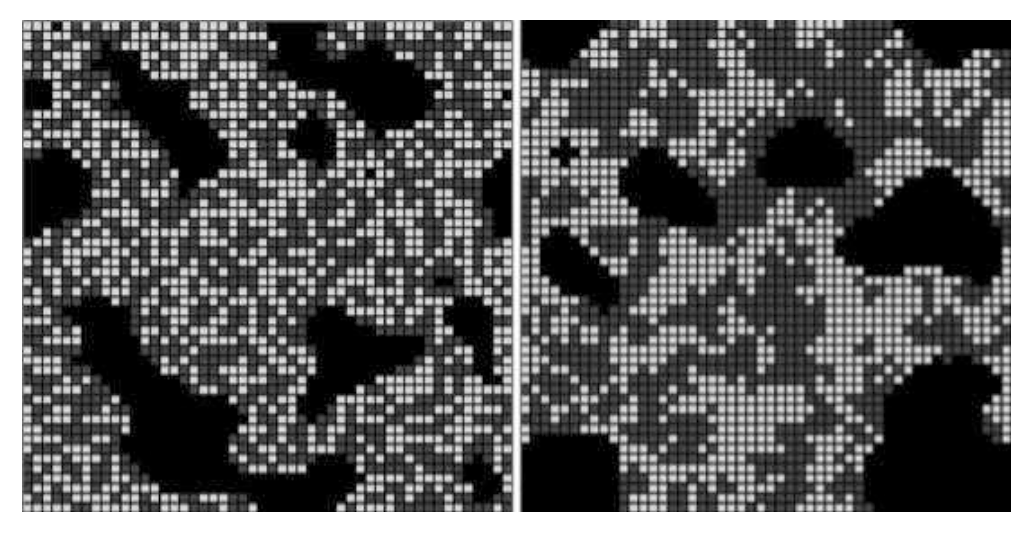
\includegraphics[width = \textwidth]{wouter3.png}
         \caption{Pattern of intergroup contact between agents with equal and
         mutually positive attitudes towards each other. In the picture on the
         left mutual attitudes are 1.00; in the right picture the mutual
         attitudes are 0.50.}
      \end{figure}
   }
   \only<5>{
      \begin{figure}
         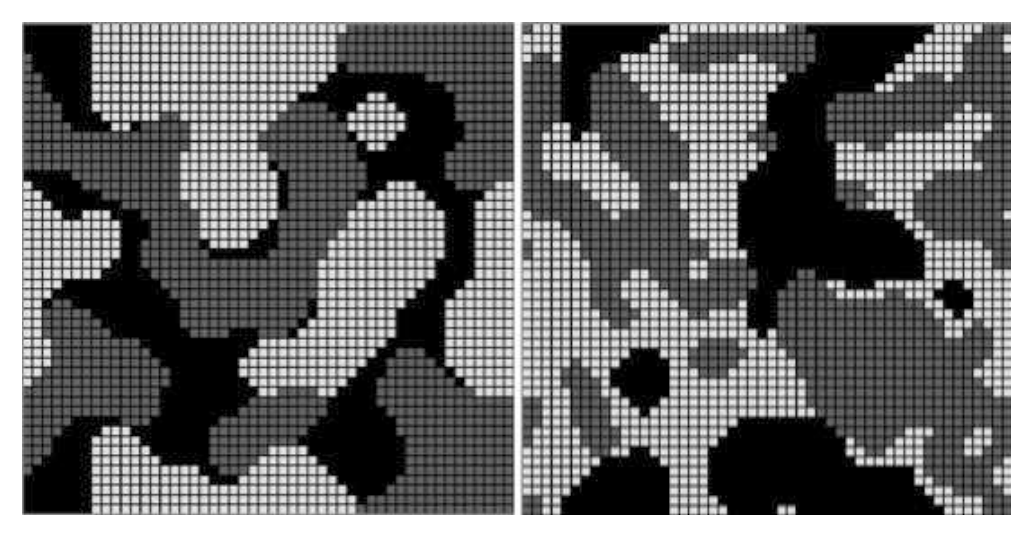
\includegraphics[width = \textwidth]{wouter4.png}
         \caption{\textbf{Left panel:} A pattern of intergroup contact between
         mutually tolerant agents; attitude towards the other group is 0.00.
         \textbf{Right panel:} the lighter shaded group has a moderately
         positive attitude of 0.50, the dark shaded group has a neutral attitude
         of 0.00.}
      \end{figure}
   }

\end{frame}
\begin{frame}
   \frametitle{Bibliography}
   \scriptsize
   \begin{enumerate}
      \item Conway, J. (1970). Conway's game of life. Scientific American.
      \item Galán, J. M., Izquierdo, L. R., Izquierdo, S. S., Santos, J. I., Del
      Olmo, R., \& López-Paredes, A. (2013). Checking Simulations: Detecting and
      Avoiding Errors and Artefacts. In B. Edmonds \& R. Meyer (Eds.),
      Simulating Social Complexity (pp. 95–116). Springer Berlin Heidelberg.
      \item De Raad, W. E., Nowak, A., \& Borkowski, W. (2013). Modeling
      Dynamics of Multicultural Integration and Conflict. In K. Sycara, M.
      Gelfand, \& A. Abbe (Eds.), Models for Intercultural Collaboration and
      Negotiation (Vol. 6, pp. 183–197). Springer Netherlands.
      \item Epstein, J. M. (2008) "Why Model?" Journal of Artificial Societies and Social Simulation, 11(4), 12.
      \item Goldstone, R. L., \& Janssen, M. A. (2005). Computational models of collective behavior. Trends in Cognitive Sciences, 9(9), 424-430.
      \item Norman, D. A. (1983). Some observations on mental models. In D. Gentner \& A. L. Stevens (Eds), Mental models, pp . 7-14. Hillsdale, NJ: Erlbaum.
      \item Schelling, T. C. (1971). DYNAMIC MODELS OF SEGREGATION. Journal of
      Mathematical Psychology, 1, 143–186.
      \item Timpone, R. J., \& Taber, C. S. (1996). Computational Modeling. London: SAGE.
   \end{enumerate}
\end{frame}

\end{document}